\section{Experiments}
\label{sec:experiments}

\subsection{Experimental Setup}
\label{sec:exp:setup}

\myparagraph{Architecture \& Implementation.}
% Tempo's local SVLM are initialized from Qwen3-VL-2B-Instruct~\cite{bai2025qwen3}, while the global LLM uses Qwen3-LM-4B. A linear projector bridges the SVLM's memory space to the LLM, yielding a compact 6B-parameter architecture.
Tempo's local SVLM is initialized from Qwen3-VL-2B-Instruct, while the global LLM uses Qwen3-LM-4B. A linear projector bridges the SVLM's memory space to the LLM, yielding a compact 6B-parameter architecture.
%
We extract frames at 2 FPS via Decord, applying uniform subsampling if limits are exceeded. During training, continuous videos are partitioned into 4-frame segments, each compressed by the SVLM into $k_{\max}=128$ memory tokens. During inference, we expand the segment window to 8 frames. ATA (Sec.~\ref{sec:method:ata}) strictly enforces a global visual budget $B_{\max}$ (4K or 8K) via head truncation. Models are trained on a 64-GPU cluster with FSDP. Additional hyper-parameters are provided in the Appendix~\ref{supp:training_details}.

\myparagraph{Progressive Training Curriculum.}
We adopt a rigorous four-stage progressive training curriculum to ensure stable optimization and context extrapolation:
% \vspace{-1em}
% \begin{itemize}
%     % \setlength{\itemsep}{2pt}
%     \item \textbf{Stage 0 (Modality Alignment):} We freeze the entire SVLM and the LLM, exclusively optimizing the linear projector using the standard LCS-558K dataset~\cite{liu2023visual}. This establishes basic vision-language alignment between the SVLM's output and the LLM's text space. 
%     \item \textbf{Stage 1 (Pre-training):} We unfreeze the entire architecture and optimize it on a large-scale multimodal corpus comprising $\sim$2M image~\cite{an2025llava}, $\sim$1.38M video~\cite{an2025llava,monfort2021spoken,kay2017kinetics,sharegemini,yang2024vript,zhang2024direct}, and $\sim$143K pure text samples~\cite{an2025llava}. Videos are sampled at 8 frames, endowing the LLM with initial temporal perception.
%     \item \textbf{Stage 2 (Broad Supervised Fine-Tuning (SFT)):} To develop robust instruction-following and semantic-aware temporal reasoning skills, we perform comprehensive SFT using a diverse data mixture ($\sim$0.93M images~\cite{an2025llava,kahou2017figureqa,ainslie2023gqa,kafle2018dvqa,lu2022dynamic,mathew2022infographicvqa,lu2022learn,masry2022chartqa,schwenk2022okvqa,biten2019scene,zhang2023llavar,textocr-gpt4v,sidorov2020textcaps,chen2024allava}, $\sim$2.25M videos~\cite{li2024videochat,zhang2024direct,wu2025large,song2024moviechat,yi2019clevrer,goyal2017something,rohrbach2017movie,liu2019ntu,patraucean2023perception,grauman2022ego4d,jang2019video,xiao2021next,wu2024star,tang2019coin,hendricks2018localizing,zala2023hierarchical,huang2020multimodal}, and $\sim$71K text samples). In this stage, the maximum number of sampled frames per video is strictly capped at 128.
%     \item \textbf{Stage 3 (Long-Context SFT):}
%     To extrapolate context length, we freeze the local compressor and exclusively fine-tune the LLM on a $\sim$384K high-quality subset from Stage 2, increasing the maximum frame limit to 384.
% \end{itemize}
% \begin{itemize}
%     % \setlength{\itemsep}{2pt}
%     \item \textbf{Stage 0 (Modality Alignment):} We freeze the entire SVLM and the LLM, exclusively optimizing the linear projector using the standard LCS-558K dataset~\cite{liu2023visual}. This establishes basic vision-language alignment between the SVLM's output and the LLM's text space. 
%     \item \textbf{Stage 1 (Pre-training):} We unfreeze the entire architecture and optimize it on a large-scale multimodal corpus comprising $\sim$2M image, $\sim$1.38M video, and $\sim$143K pure text samples. Videos are sampled at 8 frames, endowing the LLM with initial temporal perception.
%     \item \textbf{Stage 2 (Broad Supervised Fine-Tuning (SFT)):} To develop robust instruction-following and semantic-aware temporal reasoning capabilities, we perform comprehensive SFT using a diverse data mixture ($\sim$0.93M images, $\sim$2.25M videos, and $\sim$71K text samples). In this stage, the maximum number of sampled frames per video is strictly capped at 128.
%     \item \textbf{Stage 3 (Long-Context SFT):}
%     To extrapolate context length, we freeze the SVLM
%     and exclusively fine-tune the LLM on a $\sim$384K high-quality subset from Stage 2, increasing the maximum frame limit to 384.
% \end{itemize}
\begin{itemize}
    \item \textbf{Stage 0 (Modality Alignment):} We freeze both the SVLM and the LLM, exclusively optimizing the linear projector on the standard LCS-558K dataset~\cite{liu2023visual}. This establishes the fundamental vision-language alignment, bridging the SVLM's visual representations with the LLM's text embedding.
    
    \item \textbf{Stage 1 (Pre-training):} We unfreeze the entire architecture and optimize it on a large-scale, curated multimodal corpus comprising $\sim$2M images, $\sim$1.38M videos, and $\sim$143K pure text samples. During this phase, videos are sparsely sampled at 8 frames, endowing the model with initial temporal perception.
    
    \item \textbf{Stage 2 (Broad Supervised Fine-Tuning):} To develop robust instruction-following and semantic-aware temporal reasoning capabilities, we perform comprehensive SFT using a highly diverse data mixture ($\sim$0.93M images, $\sim$2.25M videos, and $\sim$71K text samples). In this stage, the temporal context is systematically expanded, with the maximum number of sampled frames per video strictly capped at 128.
    
    \item \textbf{Stage 3 (Long-Context SFT):} To effectively extrapolate the context window, we freeze the SVLM and exclusively fine-tune the global LLM on a high-quality subset of $\sim$384K samples from Stage 2. Here, the maximum frame limit is extended to 384, enabling the LLM to handle long temporal sequences.
    
\end{itemize}
%
To curate our training data, we primarily follow the data mixtures established by VideoChat-Flash~\cite{li2024videochat} and LLaVA-OneVision-1.5~\cite{an2025llava}. All training datasets utilized throughout our progressive curriculum are publicly accessible, ensuring full reproducibility.
% Dataset split statistics and the detailed list of sources are provided in the supplementary material.

\paragraph{\textbf{Evaluation Benchmarks \& Baselines.}}
To evaluate Tempo's long video understanding, we conduct comprehensive experiments across four prominent benchmarks, \ie, LongVideoBench~\cite{wu2024longvideobench}, MLVU~\cite{zhou2025mlvu}, Video-MME~\cite{fu2025video}, LVBench (extreme-long video)~\cite{wang2025lvbench}, spanning standard long-form tasks to hour-long stress tests. We benchmark Tempo against widely adopted proprietary baselines (\eg, GPT-4o, Gemini Pro 1.5), general open-weight MLLMs (\eg, InternVL, Qwen-VL), and specialized long-video MLLMs (\eg, VideoChat-Flash, LongVA). All evaluations are conducted using the \texttt{lmms-eval}.

\begin{table*}[t]
    \centering
    \setlength{\tabcolsep}{8pt} 
    \renewcommand{\arraystretch}{1.2} 
    \caption{\textbf{Comparison with state-of-the-art MLLMs on long video benchmarks, highlighting Tempo's superior accuracy and extreme token efficiency.} \textbf{Bold} and \underline{underline} denote the best and second-best results among specialized long video MLLMs. ``-'' indicates unavailable results. * indicates the average tokens per frame are dynamically adjusted. For our model, we report the theoretical dynamic range (0.5--16) alongside the actual empirical average tokens per frame ({\setlength{\fboxsep}{1pt}\colorbox{gray!10}{\textbf{gray rows}}}), demonstrating that Tempo inherently operates substantially below the maximum budget limits in practice.}
    \label{tab:main_table}
    \resizebox{\linewidth}{!}{
    \begin{tabular}{l c c ccccc}
        \toprule
        \multirow{2.5}{*}{\textbf{Model}} & \multirow{2.5}{*}{\textbf{Size}} & \textbf{Tokens} & \textbf{LongVideoBench} & \textbf{MLVU} & \multicolumn{2}{c}{\textbf{Video-MME (w/o sub.)}} & \textbf{LVBench} \\
        \cmidrule(lr){6-7}
        & & \textbf{per frame} & (473s) & (651s) & Overall (1010s) & Long (2386s) & (4101s) \\
        \midrule
        
        \addlinespace[0.3ex] 
        \multicolumn{8}{l}{\textit{Proprietary Models}} \\
        \addlinespace[0.3ex] 
        GPT-4o~\cite{hurst2024gpt}             &  - &  - & 66.7 & 64.6 & 71.9 & 65.3 & 30.8 \\
        Gemini 1.5 Pro~\cite{team2024gemini}   &  - &  - & 64.0 & -    & 75.0 & 67.4 & 33.1 \\
        \midrule
        
        \addlinespace[0.3ex]
        \multicolumn{8}{l}{\textit{General Open-Source MLLMs}} \\
        \addlinespace[0.3ex]
        VideoChat2-HD~\cite{li2025videochat}    & 7B & 72   & -    & 47.9 & 45.3 & 39.8  & - \\
        LLaVA-OneVision~\cite{li2024llava}      & 7B & 196  & 56.4 & 64.7 & 58.2 & -     & - \\
        LLaVA-Video~\cite{zhang2024llava}       & 7B & 676  & 58.2 & 70.8 & 63.3 & -     & - \\
        VideoLLaMA3*~\cite{zhang2025videollama} & 7B & $\le$ 91 & 59.8 & 73.0 & 66.2 & 54.9 & 45.3 \\
        InternVL3.5~\cite{wang2025internvl3}    & 8B & 256  & 62.1 & 70.2 & 66.0 & -    & - \\
        Molmo2~\cite{clark2026molmo2}           & 8B & 83   & 67.5 & -    & 69.9 & -    & 52.8 \\
        Qwen2.5-VL~\cite{bai2025qwen3}          & 7B & 1924 & 56.0 & 70.2 & 65.1 & -    & 45.3 \\
        Qwen3-VL*~\cite{bai2025qwen3}           & 2B & $\le$ 640 & -    & 68.3 & 61.9 & -    & 47.4 \\
        Qwen3-VL*~\cite{bai2025qwen3}           & 8B & $\le$ 640 & -    & 78.1 & 71.4 & -    & 58.0 \\
        \midrule
        
        \addlinespace[0.3ex]
        \multicolumn{8}{l}{\textit{Specialized Long Video MLLMs}} \\
        \addlinespace[0.3ex]
        LLaMA-VID~\cite{li2024llama}       & 7B   & 2   & -    & 33.2 & 25.9  & -   & 23.9 (13B) \\
        LongVA~\cite{zhang2024long}        & 7B   & 144 & -    & 56.3 & 52.6 & 46.2 & - \\
        Kangaroo~\cite{liu2024kangaroo}    & 8B   & 256 & 54.8 & 61.0 & 56.0 & 46.7 & 39.4 \\
        LongLLaVA~\cite{wang2024longllava} & A13B & 144 & 53.5 & -    & 53.8 & 46.4 & - \\
        LongVILA~\cite{chen2024longvila}   & 7B   & 196 & 57.1 & -    & 60.1 & 47.0 & - \\
        LongVU~\cite{shen2024longvu}       & 7B   & 64  & -    & 65.4 & 60.6 & 59.5 & - \\
        Storm~\cite{jiang2025storm}        & 7B   & 64  & 60.5 & 72.9 & 63.4 & 53.4 & - \\
        BIMBA~\cite{islam2025bimba}        & 7B   & 36 & 59.5 & 71.4 & 64.7 & -    & - \\
        VideoChat-Flash~\cite{li2024videochat}  & 7B  & 16   & \underline{64.7} & 74.7 & 65.3 & 55.4 & 48.2 \\
        % \rowcolor{gray!10} \textbf{Tempo* (4K Budget)} & \textbf{6B}& \textbf{0.5--16} & 64.5          & \textbf{75.6}    &  \textbf{67.8}      & \textbf{57.8}    & \textbf{52.7} \\
        % \rowcolor{gray!10} \textbf{Tempo* (8K Budget)} & \textbf{6B}& \textbf{0.5--16} & \textbf{65.1} & \underline{75.2} & \underline{67.7}   & \underline{57.0} & \underline{52.3} \\
        \midrule
        \rowcolor{gray!10} \textbf{Tempo* (4K Budget)} & \textbf{6B} & \textbf{0.5--16} & 64.5 & \textbf{75.6} & \textbf{67.8} & \textbf{57.8} & \textbf{52.7} \\
        
        \rowcolor{gray!10} \multicolumn{3}{r}{\textit{\textcolor{darkgray}{$\hookrightarrow$ actual avg. toks/frame}}} & \textit{\textcolor{darkgray}{2.8}} & \textit{\textcolor{darkgray}{2.8}} & \textit{\textcolor{darkgray}{3.6}} & \textit{\textcolor{darkgray}{3.4}} & \textit{\textcolor{darkgray}{2.9}} \\

        \midrule
        \rowcolor{gray!10} \textbf{Tempo* (8K Budget)} & \textbf{6B} & \textbf{0.5--16} & \textbf{65.1} & \underline{75.2} & \underline{67.7} & \underline{57.0} & \underline{52.3} \\
        
        \rowcolor{gray!10} \multicolumn{3}{r}{\textit{\textcolor{darkgray}{$\hookrightarrow$ actual avg. toks/frame}}} & \textit{\textcolor{darkgray}{3.1}} & \textit{\textcolor{darkgray}{3.3}} & \textit{\textcolor{darkgray}{4.3}} & \textit{\textcolor{darkgray}{4.1}} & \textit{\textcolor{darkgray}{3.5}} \\
        \bottomrule
    
    \end{tabular}
    }
\end{table*}
\subsection{Long Video Understanding}
\label{sec:main_results}

Tab.~\ref{tab:main_table} summarizes the evaluation of Tempo (capped at 1024 frames) against state-of-the-art MLLMs across four major benchmarks. Despite a compact 6B-parameter architecture and aggressive token compression (0.5--16 tokens/frame), Tempo achieves state-of-the-art performance. While larger open-weight models (\eg, Qwen3-VL 8B, Molmo2) yield strong absolute scores via exorbitant visual token consumption, Tempo operates under extreme efficiency. By routing evidence through ATA, Tempo strictly bounds visual tokens to 4K or 8K budgets. In practice, ATA dynamically distributes bandwidth so efficiently that the actual consumption falls well below these limits (\eg, 2.9 tokens/frame on LVBench under the 4K budget). Remarkably, its comparative advantage over specialized long video MLLMs amplifies as the temporal span extends.

\myparagraph{Dominance in Ultra-Long Video Understanding.}
%
The most notable results emerge on the extreme-long benchmark LVBench, a rigorous stress test for long-term memory and evidence retrieval. Operating strictly within a 4K visual budget, Tempo achieves \textbf{52.7}, outperforming the strongest 7B specialized MLLM, VideoChat-Flash (48.2), by 4.5 points. Impressively, despite its compact capacity, Tempo eclipses proprietary systems in this ultra-long setting, surpassing GPT-4o (30.8) and Gemini 1.5 Pro (33.1) by massive margins.
% 
This proves that explicit query-aware compression is vastly superior to blindly feeding raw frames into expansive LLM context windows, which often suffer from attention dilution.

\myparagraph{Robustness Across Varied Temporal Contexts.}
%
This dominance consistently extends across other benchmarks. On Video-MME, Tempo secures \textbf{67.8} under the 4K budget, exceeding VideoChat-Flash (65.3) and showing massive improvement over its base model Qwen3-VL-2B (61.9). On the challenging Video-MME \textit{Long} subset (2386s), Tempo achieves \textbf{57.8}. Similarly, Tempo delivers SOTA-level performances on MLVU (\textbf{75.6}) and LongVideoBench (\textbf{65.1} under 8K), asserting its robust generalization across diverse temporal scales and tasks.


\myparagraph{{The ``Less is More'' Phenomenon.}} 
%
Crucially, Tempo's performance under the 4K budget frequently matches or exceeds the 8K budget (\eg, 52.7 vs. 52.3 on LVBench; 57.8 vs. 57.0 on Video-MME \textit{Long} subset). This counter-intuitive phenomenon powerfully validates our ATA strategy. Enforcing a stricter information bottleneck filters out background distractors, forcing the LLM to focus purely on high-value semantic beats. This actively mitigates the \emph{lost-in-the-middle} phenomenon without requiring additional inference compute.

\myparagraph{Qualitative Analysis.}
%
We provide comprehensive qualitative results in Appendix~\ref{supp:qualitative} to further analyze Tempo's adaptive behavior. We contrast localized queries (requiring pinpoint accuracy) with global queries (requiring holistic understanding). These comparisons explicitly demonstrate how Tempo dynamically shifts its compression rhythm---allocating high-fidelity bandwidth to query-critical moments while applying extreme sparsity to irrelevant backgrounds. Crucially, for overarching queries lacking singular salient events, ATA gracefully defaults to a smooth, low-variance token allocation, ensuring global temporal comprehension remains intact.


\begin{table}[t]
    \centering
    \caption{\textbf{Ablation studies on Tempo's core components.} We decompose our framework across five dimensions: (A) progressive training curriculum, (B) segment-level budget allocation, (C) intra-segment token reduction scheme, (D) relevance scoring source, and (E) temporal continuity. Unless otherwise specified, all variants process videos uniformly sampled at 2 FPS up to a maximum of 1024 frames, strictly bounded by an 8K visual token budget for fair comparison. The default Tempo configuration is highlighted in {\setlength{\fboxsep}{1pt}\colorbox{gray!10}{\textbf{gray}}}. LongVB denotes LongVideoBench.}
    \label{tab:ablation_main}
    \setlength{\tabcolsep}{9pt}
    \resizebox{\linewidth}{!}{
    \begin{tabular}{l c c c c c}
        \toprule
        \multirow{2}{*}{\raisebox{-1.5ex}{\textbf{Ablation Setting}}} & \textbf{LongVB} & \textbf{MLVU} & \multicolumn{2}{c}{\textbf{Video-MME (w/o sub.)}} & \textbf{LVBench} \\
        \cmidrule(lr){4-5}
        & (473s) & (651s) & \begin{tabular}{@{}c@{}}\textbf{Overall} \\ (1010s)\end{tabular} & \begin{tabular}{@{}c@{}}\textbf{Long} \\ (2386s)\end{tabular} & (4101s) \\
        \midrule
        
        \multicolumn{6}{l}{\textit{A. Progressive Training Curriculum}} \\
        w/o Stage 3 - Long-Context SFT (16K Budget)        & 61.4 & 67.2 & 66.1 & 56.3 & 47.3 \\
        w/o Adaptive Token Allocation (16K Budget)         & 62.8 & 73.5 & 67.0 & 56.2 & 51.1 \\
        \rowcolor{gray!10} Tempo Default (8K Budget)       & \textbf{65.1} & \textbf{75.2} & \textbf{67.7} & \textbf{57.0} & \textbf{52.3} \\
        \midrule
        
        \multicolumn{6}{l}{\textit{B. Segment-Level Budget Allocation}} \\
        Uniform Subsampling (Equal tokens per segment)      & 61.9 & 74.0 & 66.3 & 55.2 & 49.9 \\
        Random Drop (Uniform random segment selection)      & 59.3 & 70.9 & 63.6 & 55.2 & 49.8 \\
        Adversarial Routing (Keep lowest-scoring segments)  & 50.7 & 59.3 & 52.4 & 47.8 & 36.9 \\ 
        Hard Top-K Routing (Keep highest-scoring segments)  & 63.5 & 73.9 & 66.7 & 56.2 & 52.7 \\
        \rowcolor{gray!10} ATA (Adaptive token allocation, Alg.~\ref{alg:ata}) & \textbf{65.1} & \textbf{75.2} & \textbf{67.7} & \textbf{57.0} & \textbf{52.3} \\
        \midrule

        \multicolumn{6}{l}{\textit{C. Intra-Segment Token Reduction Scheme}} \\
        Uniform Tail Truncation (Fixed 64 tokens)              & 59.5 & 71.6 & 64.1 & 54.8 & 41.8 \\
        Uniform Head Truncation (Fixed 64 tokens)              & 63.2 & 73.4 & 66.9 & 56.2 & 51.5 \\ 
        Token Merging (Merge visual features to $k_i$ tokens)  & 63.6 & 74.9 & 66.3 & 55.4 & 53.0 \\
        Dynamic Tail Truncation (Keep last $k_i$ tokens)       & 61.9 & 73.4 & 64.8 & 54.2 & 50.5 \\
        \rowcolor{gray!10}Dynamic Head Truncation (Keep first $k_i$ tokens) & \textbf{65.1} & \textbf{75.2} & \textbf{67.7} & \textbf{57.0} & \textbf{52.3} \\
        \midrule
        
        \multicolumn{6}{l}{\textit{D. Relevance Scoring Source \& Zero-Shot Prior}} \\
        Base Model Prior (Standard prompt)                              & 64.6 & 75.1 & 67.2 & 56.1 & 52.6 \\
        Base Model Prior (Explicit routing prompt)                      & 65.7 & 76.3 & 67.6 & 57.3 & 52.7 \\
        External Dense Retriever (Qwen3-VL Reranker) & 64.3 & 75.4 & 67.2 & 57.0 & 51.8 \\
        Tempo SVLM Prior (Standard prompt)                               & 64.1 & 75.4 & 67.2 & 57.0 & 53.4 \\
        \rowcolor{gray!10} Tempo SVLM Prior (Explicit routing prompt)    & \textbf{65.1} & \textbf{75.2} & \textbf{67.7} & \textbf{57.0} & \textbf{52.3} \\
        \midrule

        \multicolumn{6}{l}{\textit{E. Temporal Continuity (Minimum Token Guarantee)}} \\
        Hard Pruning (0 tokens for irrelevant segments)            & 63.9 & 74.8 & 67.4 & 56.3 & 52.3 \\
        \rowcolor{gray!10} Minimal Temporal Anchors ($k_{\min}=4$) & \textbf{65.1} & \textbf{75.2} & \textbf{67.7} & \textbf{57.0} & \textbf{52.3} \\
        
        \bottomrule
    \end{tabular}
    }
    \vspace{-1.0em}
\end{table}

\subsection{Ablation Studies}
\label{sec:exp:ablation}

\begin{figure}[t]
    \centering
    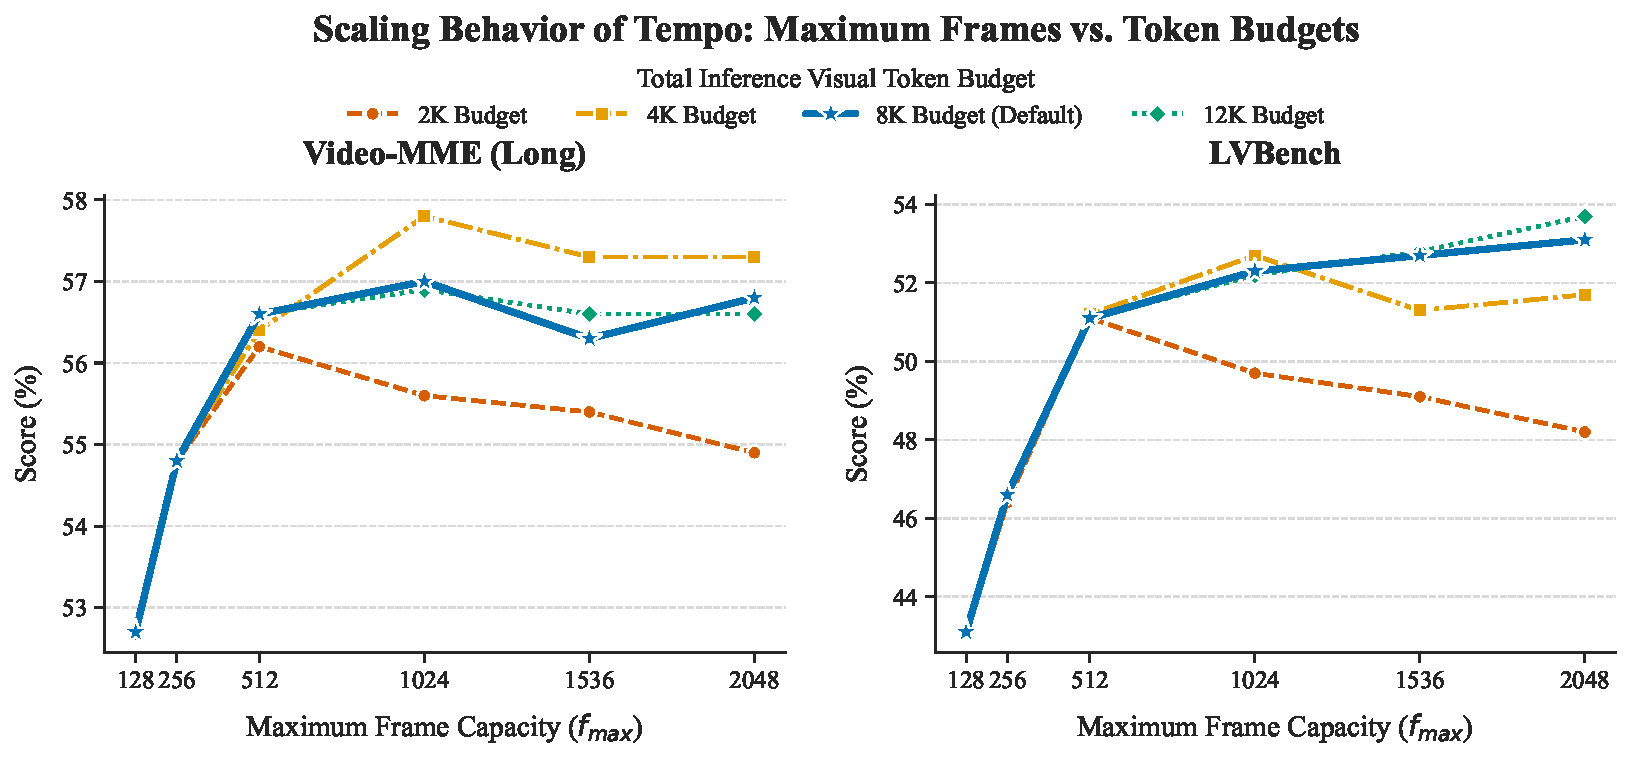
\includegraphics[width=\textwidth]{fig/scaling_behavior.pdf}
    \caption{\textbf{Scaling behavior of Tempo.} We investigate the interplay between maximum frame capacity ($f_{\max}$) and total visual token budgets. \textbf{(Left)} On Video-MME (Long), a strict 4K budget acts as an optimal \emph{sweet spot} by aggressively filtering redundancy, whereas larger budgets (8K/12K) yield marginal noise. \textbf{(Right)} On the extreme-long LVBench, restrictive budgets eventually limit the achievable performance, whereas expansive capacities (\eg, 12K) monotonically unlock new peaks at higher frame densities, proving the necessity of scaled context for hour-long video understanding.}
    % \vspace{-1.5em}
    \label{fig:scaling_behavior}
\end{figure}
% We systematically decompose Tempo's core components in Tab.~\ref{tab:ablation_main}. Unless specified, all variants process up to 1024 frames under a strict 8K visual token budget.
We systematically decompose Tempo's core components in Tab.~\ref{tab:ablation_main}. Unless specified, all variants process videos uniformly sampled at 2 FPS for a maximum of 1024 frames, strictly bounded by an 8K visual token budget.

\myparagraph{A. Progressive Training Curriculum.} 
%
We first evaluate our training stages (Tab.~\ref{tab:ablation_main}A). Stopping after Stage 2 (w/o Long-Context SFT) yields sub-optimal performance on extreme-long benchmarks (\eg, 47.3 on LVBench), as the LLM fails to extrapolate its temporal window. Introducing Stage 3 without adaptive allocation improves this to 51.1, despite a 16K budget. Crucially, combining the full curriculum with ATA achieves peak performance (52.3 on LVBench) while consuming only half the visual budget (8K). This confirms that extending context is not merely about scaling length, but maximizing information density.

\myparagraph{B. Segment-Level Budget Allocation.} 
%
To strictly satisfy the 8K token budget, all baselines fix the segment capacity at $k_{\max}$ (128) tokens. Given our sampling rate of 2 FPS (capped at a maximum of 1024 frames), Uniform Subsampling halves the initial input frames (processing up to 512 frames). In contrast, Random Drop and the routing variants process all sampled frames (up to 1024) but discard 50\% of the segments to meet the budget (Tab.~\ref{tab:ablation_main}B).
%
Notably, when we adversarially route by retaining only the lowest-scoring 50\% (Adversarial Routing), performance catastrophically collapses (\eg, 65.1 $\rightarrow$ 50.7 on LongVideoBench). This validates that our zero-shot relevance scores accurately isolate query-critical evidence. Furthermore, while Hard Top-K Routing (dropping the lowest-scoring half entirely) performs competitively, ATA outperforms it by dynamically scaling budgets and preserving overarching causality in most cases.

\myparagraph{C. Intra-Segment Token Reduction.} 
%
We next evaluate the mechanism for token reduction (Tab.~\ref{tab:ablation_main}C). Whether applying a fixed 64-token limit (Uniform) or utilizing our ATA-assigned budgets (Dynamic), Head Truncation consistently eclipses Tail Truncation (\eg, 63.2 vs. 59.5 for Uniform, and 65.1 vs. 61.9 for Dynamic on LongVideoBench). This corroborates our \emph{semantic front-loading} hypothesis (Sec.~\ref{sec:method:ata}): the causal SVLM natively packs the most critical semantics into its earliest memory tokens.
%
While Token Merging (ToMe) yields a marginal gain on LVBench (53.0 vs. 52.3), it introduces $O(N^2)$ spatial clustering overhead and degrades performance on shorter benchmarks (\eg, 66.3 vs 67.7 on Video-MME). The $O(1)$ dynamic head truncation strikes the optimal balance, offering superior generalizability with strictly zero computational overhead.

\myparagraph{D. Relevance Scoring Source \& Zero-Shot Prior.}
%
We systematically investigate the origin of the relevance scores (Tab.~\ref{tab:ablation_main}D). To isolate the routing effect, all variants here utilize Tempo's compressed memory tokens for final generation, differing only in how the ATA score $s_i$ is computed.
%
Surprisingly, we observe that the official Qwen3-VL-2B checkpoint (Base Model Prior) possesses a latent yet strong zero-shot capability for relevance alignment, achieving 76.3 on MLVU. However, extracting this prior from the base model, or utilizing an External Dense Retriever (which natively scores segments but yields sub-optimal performance), necessitates a redundant, isolated forward pass per segment.
%
In contrast, our Tempo SVLM Prior extracts these accurate routing logits simultaneously during the visual compression pass. When guided by an explicit binary instruction (full prompt can be found in the Appendix~\ref{supp:prompts_ablation}), it provides superior comprehensive performance (\eg, 67.7 on Video-MME). This single-pass design capitalizes on the foundational prior with zero latency.

\myparagraph{E. Temporal Continuity.}
%
We ablate the $k_{\min}$ constraint (Tab.~\ref{tab:ablation_main}E). Compared to a Hard Pruning strategy that aggressively drops irrelevant segments to 0 tokens, enforcing Minimal Temporal Anchors (\eg, 4 tokens/segment) consistently improves performance (\eg, 63.9 $\rightarrow$ 65.1 on LongVideoBench). This demonstrates that maintaining a continuous, highly compressed timeline is essential for long-form video understanding, preventing the LLM from losing its temporal orientation and causal tracking in hour-long videos.

\myparagraph{Scaling Behavior of Inference Context.}
%
Fig.~\ref{fig:scaling_behavior} details Tempo's scaling dynamics. At low-frame regimes, all budget curves coincide. As the uncompressed token counts remain below the budget thresholds, ATA allocations are identical. As $f_{\max}$ expands, restrictive budgets (2K, 4K) naturally degrade: enforcing the $k_{\min}=4$ temporal anchor across too many segments prematurely exhausts the capacity, starving query-critical segments of representational bandwidth.
%
At high frame counts, behavior diverges by video length. Standard long-form tasks (\eg, Video-MME Long) peak at $f_{\max}=1024$ under a 4K budget. Conversely, the extreme-long LVBench necessitates scaled capacities, where expansive 8K and 12K budgets allow performance to scale monotonically, reaching \textbf{53.7} at $f_{\max}=2048$ ($B_{\max}=12$K).
%
Notably, our empirical profiling (we provide detailed token distributions in the Appendix~\ref{supp:ata_stats}) reveals that even under generous 8K or 12K ceilings, ATA's dynamic sparsity often compresses LVBench videos ($f_{\max}=1024$) to token counts substantially below the allocated budget in practice. This demonstrates a profound property: Tempo allocates bandwidth driven by semantic necessity, rather than greedily padding to fill the available context window.